\chapter{Recurrent Neural Networks}\label{ch:rnn}

\section{Recurrent Neural Networks}
\begin{figure}
	\begin{center}
		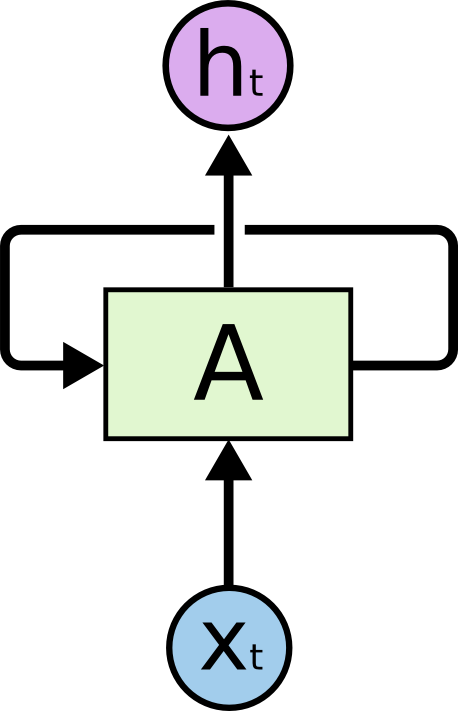
\includegraphics[scale=0.5]{rnn/rnn_rolled}
	\end{center}
	\caption{A recurrent neural network.\label{fig:rnn_img}}
	\source{http://colah.github.io/posts/2015-08-Understanding-LSTMs/img/RNN-rolled.png}
\end{figure}

A recurrent neural network (RNN) is a variation of artificial neural networks that continuously uses the output of its previous layer as the input of the current layer along with the input the user feeds into it (see figure~\ref{fig:rnn_img}). Because of this feature, RNNs have the ability to \"remember\" previous input values as they can be passed along through the previous iteration's output. 

\begin{figure}
	\begin{center}
		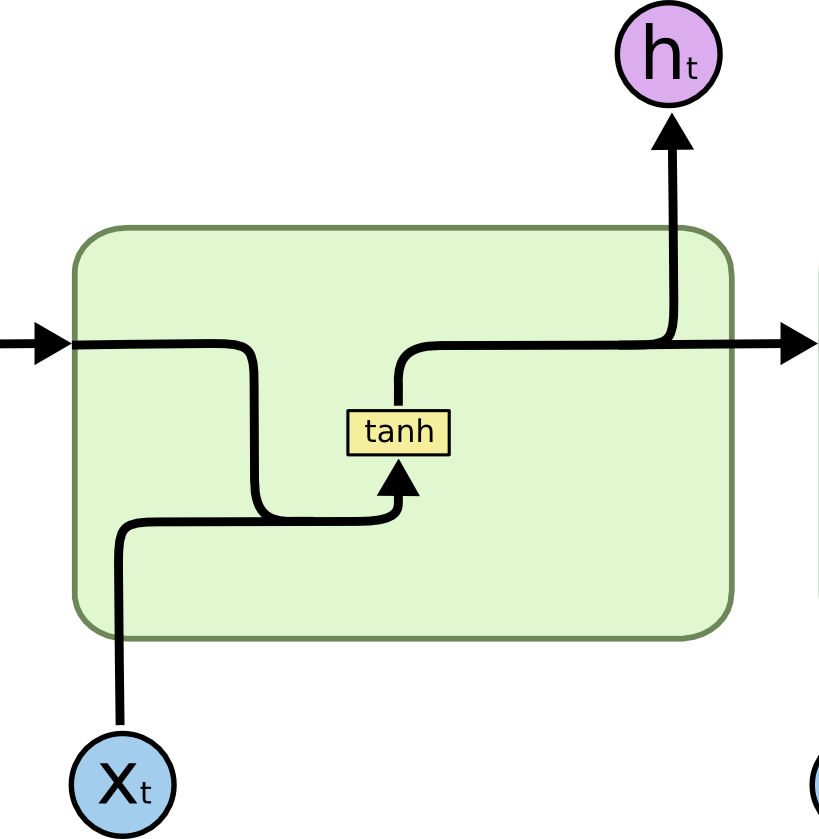
\includegraphics[scale=0.5]{rnn/rnn_cell}
	\end{center}
	\caption{A single RNN cell.\label{fig:rnn_cell}}
	\source{http://colah.github.io/posts/2015-08-Understanding-LSTMs/img/LSTM3-SimpleRNN.png}
\end{figure}

As can be seen in~\ref{fig:rnn_cell} RNNs only have a single value that acts as both the output of the cell and the data passed through to the next iteration. This hidden layer value h$_{\text{t}}$ at timestep t is calculated by the following function where h$_{\text{t}}$ is the value of the current hidden state, h$_{\text{t-1}}$ the value of the previous hidden state and so on, $W$ is the weight matrix for the cell's input, $U$ is the weight matrix for the hidden value, x$_{\text{t}}$ is the input of the cell at timestep x, and $\sigma$ is a sigmoid function used to squash its inputs into the [-1, 1] range:

\[ h_t = \sigma(Wx + Uh_\text{t-1}) \]

In theory the RNN has the ability to \"remember\" things from the past, however in practice standard RNNs seem to be not that amazing at learning. Both \cite{hochreiter1997long} and \cite{bengio1994learning} investigated this problem and found some reasons for this happening, prompting the development of the commonly used Long Short Term Memory (LSTM) RNN.

\section{LSTMs}

\begin{figure}
	\begin{center}
		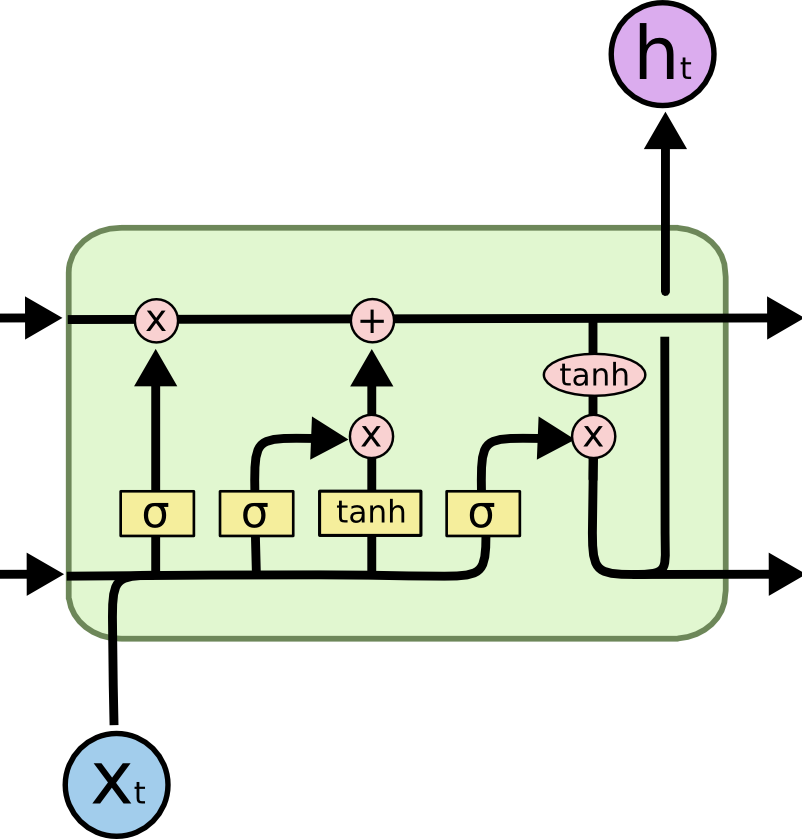
\includegraphics[scale=0.5]{rnn/lstm_cell}
	\end{center}
	\caption{A single RNN cell.\label{fig:lstm_cell}}
	\source{http://colah.github.io/posts/2015-08-Understanding-LSTMs/img/LSTM3-chain.png}
\end{figure}

Contrary to regular RNNs, LSTMs have the distinct difference of having an additional hidden state that is never directly outputted (see figure \cite{fig:lstm_cell}). This additional hidden state can then be used by the network solely for remembering relevant actions, instead of having to share its \"memory\" with its output, these values are now separate. This has the advantage of the network never having to forget things, as remembering is its default state, seeing as the line keeps going on to the next iteration.

As can be seen in the figure, there are quite a bit more parameters to this cell than a normal RNN cell. It has one weight that determines how much of its memory to \"forget\", this is also called the \"forget gate\". It also has a weight that determines how much of its 